\chapter{ComedianStrategy}\label{appendix:comedian}

\begin{figure}[htpb]
  \centering
  \begin{tabular}{c}
  \begin{lstlisting}[language=python]
    class ComedianStrategy:
        def __init__(self, threshold = 0.5):
            self.deep_comedian = DeepComedian()
            self.simple_comedian = SimpleComedian()
            self.count = 0
            self.threshold = threshold
    
        def configure(self, random: bool = False, interleaving: bool = False):
            self.random = random
            self.interleaving = interleaving
            if self.interleaving:
                self.count += 1
                if self.count % 2 == 0:
                    self.comedian = self.simple_comedian
                else:
                    self.comedian = self.deep_comedian
            elif self.random:
                if self.threshold < rand.random():
                    self.comedian = self.simple_comedian
                else:
                    self.comedian = self.deep_comedian
            else:
                self.comedian = self.deep_comedian
    
        def render(self, type: List, utterance: str) -> str:
            if self.comedian is not None:
                return self.comedian.render(type, utterance)
            else:
                logger.error("No comedian specified!")
                return ""
  \end{lstlisting}
  \end{tabular}
  \caption{The main methods of the ComedianStrategy class.}\label{fig:comedianstrategylist}
\end{figure}

\chapter{Final Affinity Scores Result}\label{appendix:finalscores}

\begin{table}[hbt!]
\centering
\begin{tabular}{|l|l|l|l|l|l|l|l|l|l|l|l|l|l|l|l|l|l|l|}
\hline
\multicolumn{19}{|c|}{Final Affinity Scores}                                         \\ \hline
User & \multicolumn{18}{c|}{Scores \{\(c_1\):\(c_{18}\)\}}                   \\ \hline
0228L160431P & 4 & 0 & 3 & 5 & 0 & 3 & 2 & 1 & 1 & 1 & 0 & 3 & 0 & 0 & 0 & 0 & 0 & 0 \\ \hline
0228Y165728S & 3 & 0 & 1 & 0 & 0 & 1 & 3 & 0 & 0 & 2 & 0 & 1 & 0 & 0 & 0 & 0 & 0 & 0 \\ \hline
0303D134007S & 0 & 2 & 2 & 1 & 0 & 1 & 1 & 1 & 2 & 0 & 0 & 1 & 2 & 0 & 2 & 1 & 0 & 2 \\ \hline
0303D161701L & 0 & 4 & 0 & 1 & 5 & 0 & 3 & 0 & 8 & 2 & 0 & 4 & 0 & 0 & 2 & 0 & 6 & 1 \\ \hline
0303J155544M & 0 & 3 & 0 & 2 & 0 & 0 & 0 & 3 & 0 & 0 & 0 & 0 & 0 & 0 & 3 & 0 & 1 & 0 \\ \hline
0303M151400P & 0 & 1 & 0 & 0 & 3 & 0 & 0 & 1 & 2 & 1 & 0 & 0 & 0 & 3 & 1 & 1 & 2 & 1 \\ \hline
0303M170134N & 0 & 1 & 1 & 0 & 1 & 2 & 1 & 2 & 2 & 3 & 1 & 1 & 2 & 1 & 1 & 2 & 0 & 3 \\ \hline
0303P142946H & 3 & 3 & 0 & 2 & 5 & 3 & 0 & 2 & 4 & 0 & 1 & 1 & 4 & 0 & 4 & 1 & 3 & 0 \\ \hline
0303P201302N & 0 & 3 & 2 & 3 & 1 & 0 & 3 & 3 & 2 & 1 & 5 & 4 & 2 & 0 & 2 & 1 & 1 & 3 \\ \hline
0303V145445S & 1 & 1 & 1 & 2 & 2 & 0 & 1 & 0 & 0 & 0 & 0 & 1 & 0 & 0 & 0 & 0 & 3 & 2 \\ \hline
0304J142142B & 1 & 0 & 0 & 0 & 0 & 0 & 0 & 0 & 0 & 0 & 0 & 0 & 0 & 0 & 0 & 4 & 1 & 1 \\ \hline
0304L200631S & 0 & 2 & 1 & 4 & 4 & 4 & 5 & 5 & 4 & 6 & 4 & 4 & 7 & 5 & 2 & 1 & 3 & 9 \\ \hline
0304M152010H & 3 & 2 & 0 & 1 & 4 & 1 & 4 & 2 & 0 & 6 & 2 & 2 & 0 & 1 & 2 & 1 & 1 & 1 \\ \hline
\end{tabular}
\caption{Final affinity scores in Funboy for all participants in after the conducted experiment.}
\label{table:fas1}
\end{table}

\chapter{EmoPy Misclassification Example}\label{appendix:emopy}

\begin{figure}[htpb]
  \centering
  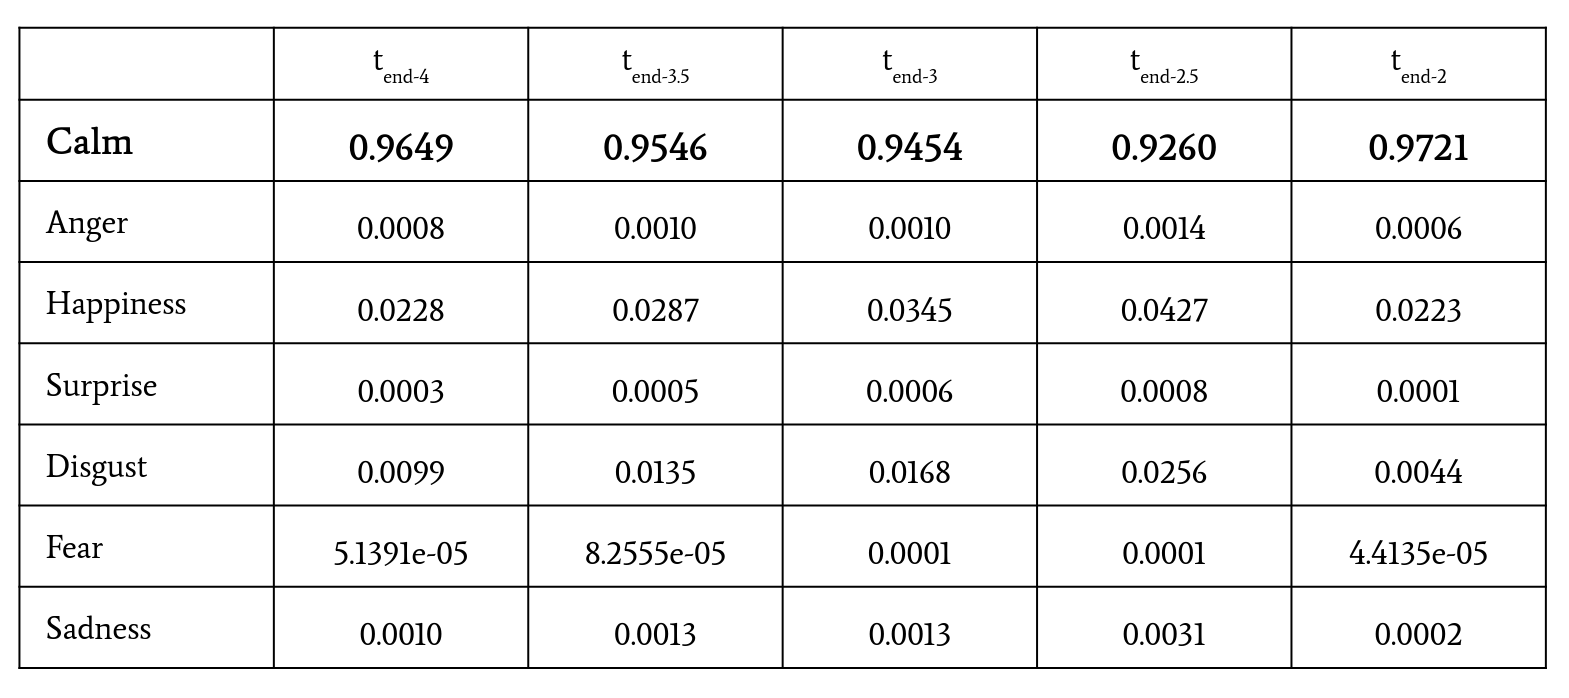
\includegraphics[width=1.0\textwidth]{figures/emopymis.png}
  \caption{Example of the VideoEmotion frame with misclassified EmoPy result.} \label{fig:vimm}
\end{figure}

